\chapter{Лінійна Класифікація та Логістична Регресія.}

\section{Лінійна Класифікація.}

Доволі поширеною задачею в машинному навчанні є задача класифікації даних. Чи є електронний лист, який ви щойно отримали, спамом? Чи схильний клієнт вашого бізнесу залишити компанію? Чи на фотографії зображена кішка, чи собака? Все це задачі класифікації даних.

Основною відмінністю задачі класифікації від задач регресії, які ми розглядали в попередньому розділі, є тип даних, які прогнозує модель. Якщо в задачі регресії модель прогнозує неперервне числове значення (згадаємо задачу про прогноз заробітньої плати працівника), то модель класифікації прогнозує категоріальний тип даних (спам чи ні, кіт чи собака, та ін.)

\begin{itemize}
\item Завдання регресії: прогнозування реальної величини $y\in R$
\item Завдання класифікації: прогнозування дискретної величини $y$
\item Бінарна класифікація: $y\in \{-1,1\}$
\item Багатокласова класифікація: $y\in \{1,2,,..., k\}$
\end{itemize}



\subsection{Приклад лінійної класифікації: класифікація раку молочної залози}

Відомий приклад класифікації: використання машинного навчання для діагностики того, чи є 
пухлина молочної залози доброякісною чи злоякісною.

Умови: лікар бере зразок рідини з пухлини, фарбує клітини, а потім окреслює 
декілька клітин (обробка зображення уточнює контури)

Система обчислює характеристики кожної клітини, такі як площа, периметр, увігнутість, текстура 
(всього 10); обчислює середнє/стандартне/максимальне значення для всіх характеристик.


\begin{lstlisting}
import numpy as np
import sklearn.datasets
import matplotlib.pyplot as plt
dat = sklearn.datasets.load_breast_cancer()

ix = np.where(dat["feature_names"] == "mean area")[0][0]
iy = np.where(dat["feature_names"] == "mean concave points")[0][0]

def plot_cells():    
    plt.scatter(dat["data"][:,ix][dat["target"]==1], dat["data"][:,iy][dat["target"]==1], marker='x', color='C0')
    plt.scatter(dat["data"][:,ix][dat["target"]==0], dat["data"][:,iy][dat["target"]==0], marker='+', color='C3')
    plt.xlim([0,2600])
    plt.ylim([0,0.21])
    plt.xlabel("Mean Area")
    plt.ylabel("Mean Concave Points")
    plt.legend(['Benign', 'Malignant'])

plot_cells()
\end{lstlisting}

Результат:

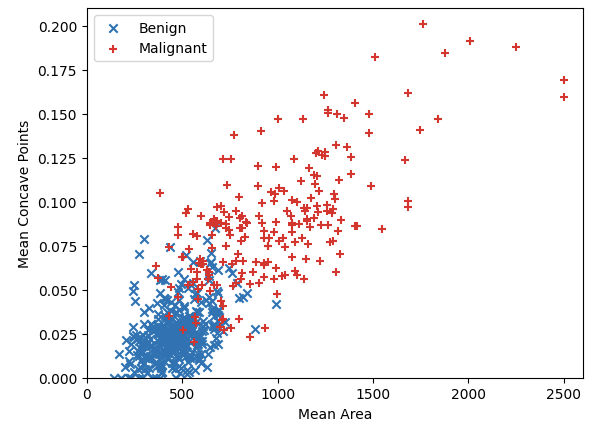
\includegraphics[scale=0.75]{img/202-1}


Задача лінійної класифікації = "Провести лінію, що розділить класи"

\subsection{Функція втрат.}

Як визначити функцію втрат (Loss function) $l:R\times \{-1, 1\}\rightarrow R$ ?
Квадратична втрата є поганою ідеєю:

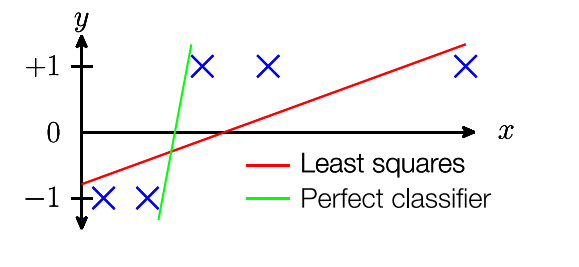
\includegraphics[scale=0.75]{img/m-class}

Ідеальна функція втрат виглядала б наступним чином:

$$l(h_{\theta}(x), y)= \begin{cases}
    0,& \text{if } sign(h_{\theta}(x))=y\\
    1,              & \text{otherwise}
\end{cases} $$

Приклади функцій втрат: logistic, hinge, exponential.

\begin{lstlisting}
hy = np.linspace(-3,3,1000)
plt.plot(hy,(hy<=0))
plt.plot(hy, np.log(1+np.exp(-hy)))
plt.plot(hy, np.maximum(1 - hy, 0))
plt.plot(hy, np.exp(-hy))
plt.xlim([-3,3])
plt.ylim([-0.05, 5])
plt.ylabel("Loss")
plt.xlabel("$h_theta(x) \cdot y$")
plt.legend(['Zero-one', 'Logistic', 'Hinge', 'Exponential'])
\end{lstlisting}

Результат:

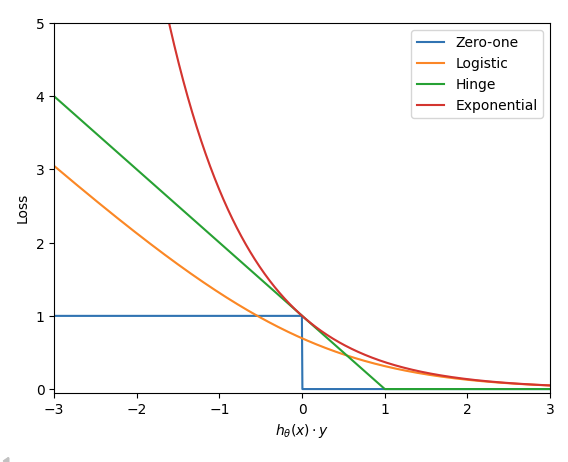
\includegraphics[scale=0.75]{img/202-2}


\section{Логістична регресія.}

Логістична регресія (Logistic regression) характерна вибором наступної функції втрат:

$$l_{logistic}(h_{\theta}(x), y) = log(1 + exp(-h_{\theta}(x)\cdot y))$$

Логістична регресія також має гарну ймовірнісну інтерпретацію: певні величини дають ймовірність, за певною моделлю, того, що приклад буде позитивним або негативним.

\begin{lstlisting}
import numpy as np
import matplotlib.pyplot as plt
from sklearn.datasets import load_breast_cancer
from sklearn.model_selection import train_test_split
from sklearn.preprocessing import StandardScaler
from sklearn.linear_model import LogisticRegression
from sklearn.metrics import confusion_matrix, ConfusionMatrixDisplay, precision_score, recall_score, f1_score, classification_report

# load data
data = load_breast_cancer()
X = data.data[:, [3, 25]]  # mean area, mean concave points
y = data.target # 0 means malignant tumor, 1 mean benign tumor

X_train, X_test, y_train, y_test = train_test_split(X, y, test_size=0.2, random_state=42, stratify=y)
scaler = StandardScaler()
X_train = scaler.fit_transform(X_train)
X_test = scaler.transform(X_test)

# fit
clf = LogisticRegression()
clf.fit(X_train, y_train)
y_pred = clf.predict(X_test)

# decision boundary grid
xx, yy = np.meshgrid(
    np.linspace(X_test[:,0].min()-1, X_test[:,0].max()+1, 300),
    np.linspace(X_test[:,1].min()-1, X_test[:,1].max()+1, 300)
)
grid = np.c_[xx.ravel(), yy.ravel()]
Z = clf.predict(grid).reshape(xx.shape)

# true labels + decision boundary
plt.contourf(xx, yy, Z, alpha=0.2, levels=[-1,0,1], colors=['C3','C0'])
# plt.scatter(X_test[:,0], X_test[:,1], c=y_test)
for cls, marker, color in [(0, '+', 'red'), (1, 'x', 'blue')]:
    idx = (y_test == cls)
    plt.scatter(
        X_test[idx, 0],
        X_test[idx, 1],
        marker=marker,
        color=color,
        label=f"Class {cls}"
    )
plt.title("True labels + decision boundary")
plt.xlabel("mean area (scaled)")
plt.ylabel("mean concave points (scaled)")
plt.show()

# confusion matrix + metrics
cm = confusion_matrix(y_test, y_pred)
disp = ConfusionMatrixDisplay(cm)
disp.plot(cmap="Blues")  
plt.title("Confusion Matrix")
plt.show()

precision = precision_score(y_test, y_pred)
recall = recall_score(y_test, y_pred)
f1 = f1_score(y_test, y_pred)

print("Precision:", precision)
print("Recall:", recall)
print("F1:", f1)

print()
print(classification_report(y_test, y_pred))
\end{lstlisting}

Результат:

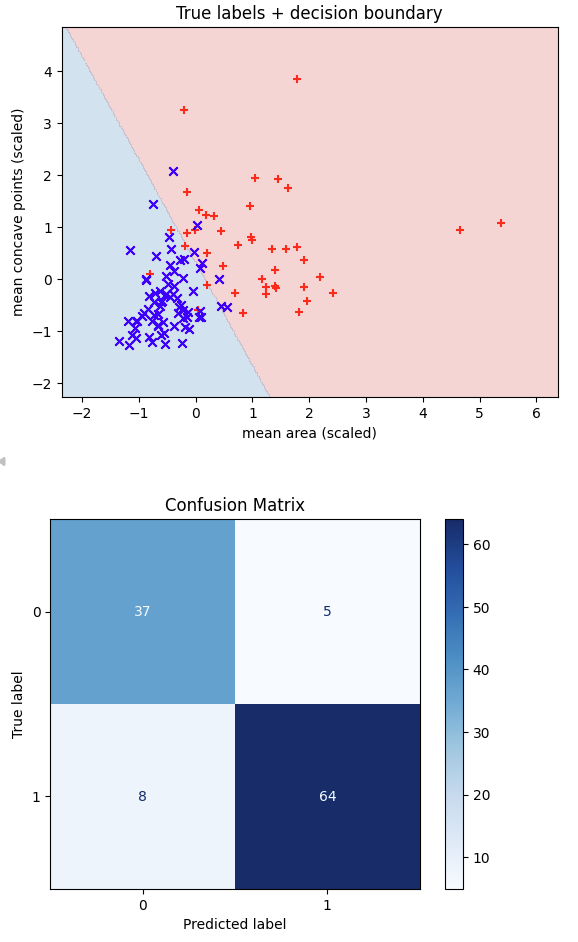
\includegraphics[scale=0.75]{img/202-3}

\begin{console}
Precision: 0.927536231884058
Recall: 0.8888888888888888
F1: 0.9078014184397163

              precision    recall  f1-score   support

           0       0.82      0.88      0.85        42
           1       0.93      0.89      0.91        72

    accuracy                           0.89       114
   macro avg       0.87      0.88      0.88       114
weighted avg       0.89      0.89      0.89       114
\end{console}

\subsection{Метрики моделей машинного навчання.}

При роботі з моделяма машинного навчання варто вміти оцінити, наскільки якісно та чи інша модель справляється з задачами, які перед нею ставляться. Як це зробити? Логічно подивитися на відношення даних, які вона класифікує правильно, до кількості неправильно класифікованих даних. 

\textit{Матриця невідповідностей (Confusion matrix)}: Це матриця розміром 2×2 для бінарної класифікації з фактичними значеннями на одній осі та прогнозованими на іншій.

Істинно позитивні (True Positive, TP) – модель правильно прогнозує позитивний клас (прогноз і фактичне значення є позитивними).

Істинно негативні (True Negative, TN) – модель правильно прогнозує негативний клас (прогноз і фактичний результат є негативними).

Хибно позитивні (False Positive, FP) – модель дає неправильний прогноз негативного класу (прогноз – позитивний, фактичний результат – негативний). (Type 1 error)

Хибно негативні (False Negative, FN) – модель дає неправильний прогноз щодо позитивного класу (прогноз – негативний, фактичний результат – позитивний). (Type 2 error)

\begin{table}[htbp]
\centering
\caption{Матриця помилок (Confusion Matrix)}
\label{tab:confusion_matrix}
\begin{tabular}{lll}
\toprule
                     & \textbf{Передбачувані позитивні} & \textbf{Передбачувані Негативні} \\ 
\midrule
\textbf{Справді Позитивні} & True Positive (TP)               & False Negative (FN)              \\ 
\textbf{Справді Негативні} & False Positive (FP)               & True Negative (TN)               \\ 
\bottomrule
\end{tabular}
\end{table}


\textit{Влучність (Precision)}: З усіх позитивних прогнозів, який відсоток є дійсно позитивним?

$$P = \frac{TP}{TP + FP}$$

\textit{Повнота (Recall)}: З загальної кількості позитивних результатів, який відсоток є прогнозованими позитивними.

$$R = \frac{TP}{TP + FN}$$

\textit{F1-міра (F1 Score)}: Це гармонійне середнє значення влучності та повноти. Воно враховує як помилкові позитивні, так і помилкові негативні результати. Тому воно добре працює з незбалансованими наборами даних.

$$F_{1} = \frac{2}{\frac{1}{P} + \frac{1}{R}}$$



\ding{46} \textbf{Питання для самоконтролю.}

\begin{enumerate}
\item Що таке класифікація в машинному навчанні?
\item Чим задачі класифікації відрізняються від задач регресії?
\item Які приклади задач класифікації можна зустріти в інтелектуальному аналізі даних?
\item Що таке лінійна класифікація?
\item Яка основна ідея лінійного класифікатора?
\item Що таке гіперплощина класифікації?
\item Як рівняння прямої використовується для поділу двох класів?
\item Що таке вагові коефіцієнти моделі класифікації?
\item Яку роль відіграє зміщення (bias) у лінійній класифікації?
\item Як інтерпретувати знак лінійної функції класифікації?
\item Які переваги має лінійна класифікація?
\item Які обмеження мають лінійні класифікатори?
\item Чому не всі задачі можна розв'язати за допомогою лінійної класифікації?
\item Як можна візуалізувати межу прийняття рішення (decision boundary)?
\item Які ознаки використовуються для класифікації раку молочної залози?
\item Чому задача класифікації раку молочної залози є бінарною?
\item Що означає правильна класифікація пацієнта?
\item Чому точність класифікації є критично важливою в медичних задачах?
\item Що таке функція втрат (Loss Function)?
\item Для чого використовується функція втрат під час навчання моделі?
\item Чому модель прагне мінімізувати значення функції втрат?
\item Чим функція втрат відрізняється від метрики якості моделі?
\item Що таке логістична регресія?
\item Чому логістична регресія, незважаючи на назву, використовується для задач класифікації?
\item Яку роль відіграє сигмоїдна (логістична) функція?
\item Які значення може приймати сигмоїдна функція?
\item Як інтерпретувати результат логістичної регресії як ймовірність належності до класу?
\item Як виконується остаточна класифікація на основі отриманої ймовірності?
\item Що таке поріг класифікації (classification threshold)?
\item Як зміна порога класифікації впливає на результати моделі?
\item Що таке матриця невідповідностей (Confusion Matrix)?
\item Які чотири типи прогнозів містить матриця невідповідностей?
\item Що означають True Positive (TP), True Negative (TN), False Positive (FP) та False Negative (FN)?
\item Що таке влучність (Precision) і як вона обчислюється?
\item Що таке повнота (Recall) і як вона обчислюється?
\item У яких випадках важливіше максимізувати Precision, а в яких — Recall?
\item Що таке F1-міра та чому вона використовується?
\item Чому однієї лише точності (Accuracy) часто недостатньо для оцінювання моделі?
\item Як інтерпретувати результати моделі за допомогою матриці невідповідностей і метрик Precision, Recall та F1?
\item Які практичні рекомендації можна дати щодо вибору метрик оцінювання для різних задач класифікації?
\end{enumerate}
